\chapter{Background and Related Work} \label{chap:background}

\section{Introduction}

The background of the object flow concept is mainly related to object tracker techniques and optical flow methods. A short state of the art review is presented in 
following sections, without going too deeply in any specific approach, since those are widely diverse. Of course, another important point is the object segmentation problem in videos. Several works have discussed this or similar problems in 
the state of the art, and only the more related approaches are presented. On the other hand, as the object flow itself is a novel problem, the related work is not large.
 However, in terms of applications, some works have been done towards specific oncomings to this concept. Some of these are superficially explained.

\section{Object Tracking}

   \begin{figure}[thpb]
      \centering
      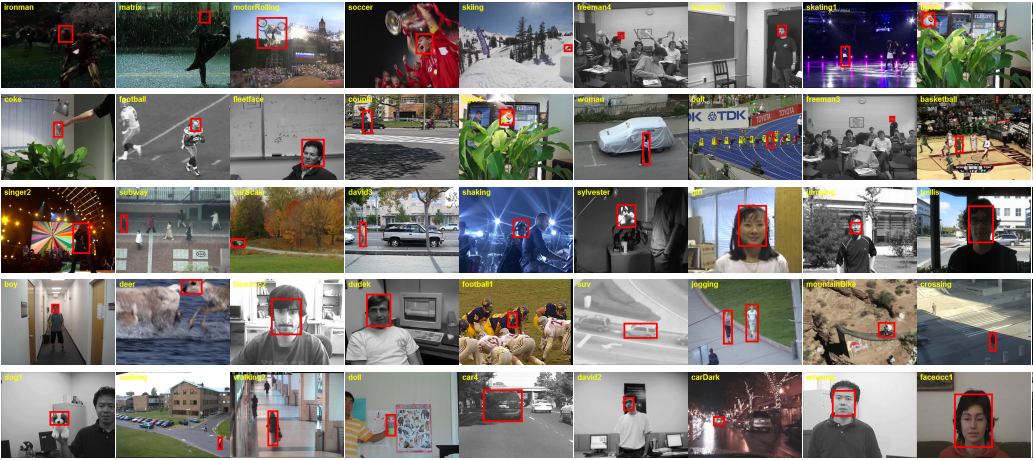
\includegraphics[width=1.0\textwidth]{../images/tr_db.png}
      \caption{Sequences used to evaluate object trackers in \cite{c16}. }
      \label{tr_db}
   \end{figure}

As one of the most studied computer vision problems, object tracking has been constantly evolving since its early approaches. 
As the techniques were getting better, the benchmarking has been evolving too. The last global work in online object tracking evaluation 
was the work of Wu et al. \cite{c16} in 2013. Several remarks can be extracted from the deep benchmarking analysis of this work. 
For instance, it seems to be more clear that background information is a key hint towards 
better tracking methods. Some kind of modelling of the background should be an important 
step in the tracking pipeline. Whether this background modelling is implicit like in \cite{c23} or 
explicit like in \cite{c22}, where is used as context, is just matter of design. Of course, this 
background modelling have to be accompanied with a local model to account with variations (occlusions, deformations) in the interest object. 
It seems that these two are the reasons why tracking by detection and learning approaches are among the most successful ones. Usually, 
these methods account with local and background modelling (\cite{c22}\cite{c23}\cite{c24}\cite{c25}\cite{c26}). 
However, even when motion or dynamical models are crucial for object tracking, very few of the last state of the art techniques focus on this 
element. The Fig. \ref{tr_per} shows results for the top 15 state of the art trackers as presented in \cite{c16}, taking into account 
the variability of different initialization. According to this data, the tracking problem is still open and further exploration can be done. 
Moreover, it has to be observed that tracking by detection methods are indeed in the top of results in stability in initialization and peak performance. 
The Struck tracker \cite{c23}, for instance, seems to hold the higher position w.r.t stability. Another curious observation is the fact that even traditionally good color based particle filter approaches are left behind by last years object trackers.

   \begin{figure}[thpb]
      \centering
      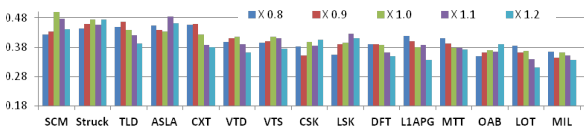
\includegraphics[width=1.0\textwidth]{../images/trackers_performance.png}
      \caption{ Performance summary for the top 15 trackers benchmarked in \cite{c16}, initialized with different size of bounding box by factors of 0.8, 0.9, 1.0, 1.1 and 1.2. }
      \label{tr_per}
   \end{figure}

\subsection{Tracking-by-detection methods}

Current tracking methods look at the problem as a classification task and use online learning techniques to update the object model \cite{c23}. The main reasons for the success of these approaches are the recent advances in object detection
methods ({\it boosting}, {\it SVM}) and fast learning algorithms. 
The normal 
pipeline of these methods includes to 
sample the image to create a list 
of labelled training examples. 

   \begin{figure}[thpb]
      \centering
      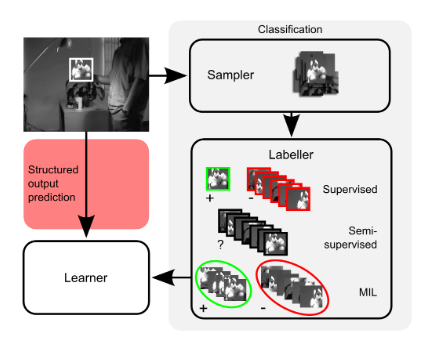
\includegraphics[width=0.66\textwidth]{../images/tbd.png}
      \caption{Usual approaches for tracking-by-detection methods. Right: generate a set of samples and, depending on the type of learner, produce training labels. Left: Structured output methods avoid these steps by operating directly in the tracking output. Extracted from \cite{c23}.}
      \label{tr_tbd}
   \end{figure}


Usually, the position of the object 
is computed from the sample with the maximum classification score in a local search window. 
This method, however, is not perfect, and most of the methods 
focus on increasing the robustness 
of the classifier to poor labelling 
and sampling, by including semi-supervised learning, robust statistics or multiple-instance 
learning \cite{c25}. Other approaches deal with these problems 
in a whole different way. For instance, the use of structured learning seems to outperform most 
of the tracking-by-detection methods \cite{c23}. In this way, 
the tracking is defined directly 
as predicting the change in object location between frames, by the use 
of structured output spaces (the same that is used in applications like text translation). Fig. \ref{tr_tbd} shows a diagram of most used approaches to tracking-by-detection methods. 
   
\section{Optical Flow}

   \begin{figure}[thpb]
      \centering
      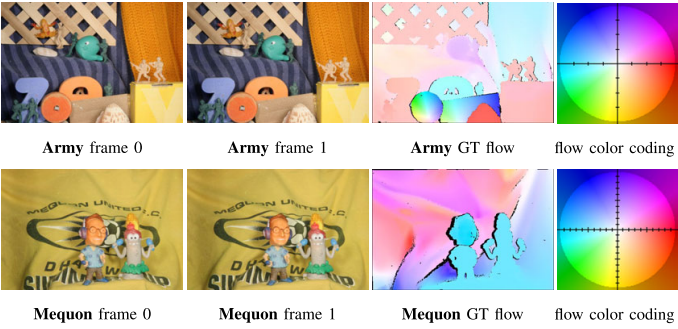
\includegraphics[width=1.0\textwidth]{../images/of_db.png}
      \caption{Frame pairs used to evaluate optical flow methods in \cite{c17}, Ground truth flow coded with the proposed flow coding. }
      \label{tr_db}
   \end{figure}

Optical flow is another traditional problem in computer vision, and it may be argued that its under-determined nature makes it one of the most difficult ones. 
Several well known databases and benchmarks have been proposed to account for the different intrinsic complications of the problem. The last and larger benchmarking 
work for this problem may be Baker et al. \cite{c17}, but other useful studies are available \cite{c27}. 
These works reveal that most of the existing methods establish the problem as the optimization of an energy function that takes into account two terms (Eq. \ref{eq_ener}). The first one, $E_{data}$ 
measures data consistency over input frames, and $E_{prior}$ which favours flow with certain characteristics, e.g. smoothness in the flow. It seems that one of the major 
challenges remains to be the best pair of objective function and optimization method. A number of combinations have been proposed \cite{c29}\cite{c30}\cite{c32}. However, 
totally different approaches had been also proposed, e.g. by using polynomial expansions \cite{c28}.

\begin{equation}
E_{global} = E_{data} + \lambda E_{prior}
\label{eq_ener}
\end{equation}

According to the update of 2011 of the work in \cite{c17}, the first 15 optical flow methods by interpolation error are shown in the Fig. \ref{of_per}. It has to be noted that the performance in several of the dataset is already very good for the most of these methods.

   \begin{figure}[thpb]
      \centering
      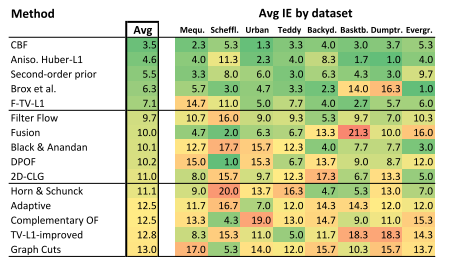
\includegraphics[width=0.8\textwidth]{../images/of_performance.png}
      \caption{ Performance summary for the top 15 opt. flow methods benchmarked in \cite{c17} by interpolation error. }
      \label{of_per}
   \end{figure}

\subsection{Simple Flow}

As the Simple Flow \cite{c21} is the optical flow technique that is used as base of the proposed 
object flow method, it is presented in more detail. 
The main characteristic of this method is its efficient approach, which tries to concentrate in the zones where there is evidence of motion, and uses linear 
interpolation for excluded zones (Fig. \ref{simple_of_m}). 
Moreover, the problem is not solved in the usual way by minimizing a variation of (\ref{eq_ener}), but using a simpler likelihood model that 
follows the constant-color assumption, without including explicitly the pairwise terms that account for smoothing. The smoothness prior it is taken into 
account, however, by implementation of local filters that uses pixel weighting to take into account pixel proximity ($w_d$) and color similarity ($w_c$), leading to the Eq. \ref{eq_simple}, which tries 
to find the vector $(u,v)$ that explain the motions in the point $(x_0,y_0)$, but also in its 
neighbourhood $\mathcal{N}_{0}$.

\begin{equation}
E(x_0, y_0, u, v) = \sum_{(x,y) \in \mathcal{N}_{0}} w_{d}w_{c}||  I_{0}(x,y) - I_{1}(x+u,y+v) ||^2
\label{eq_simple}
\end{equation}

   \begin{figure}[tbhp]
      \centering
      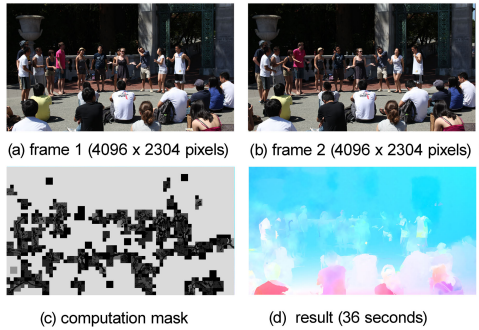
\includegraphics[width=0.85\textwidth]{../images/simpleflow.png}
      \caption{  Results of the Simple Flow method in several datasets. }
      \label{simple_of_m}
   \end{figure}

   \begin{figure}[tbhp]
      \centering
      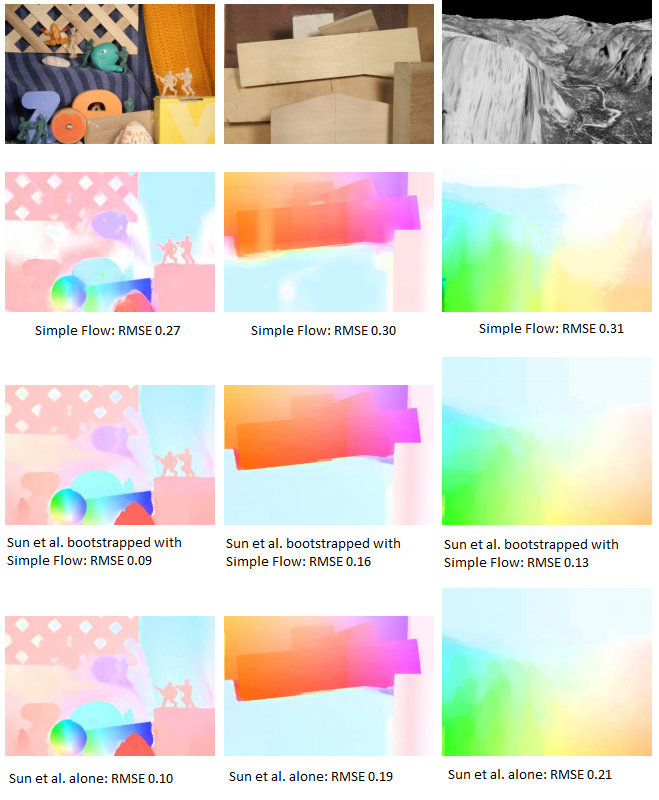
\includegraphics[width=0.95\textwidth]{../images/simpleoptflow.png}
      \caption{  Results of the Simple Flow method in several datasets. }
      \label{simple_of}
   \end{figure}

The practical implementation of this equation requires a cross-bilateral filter to compute $E$, as it takes into account 
pixel $(x_0,y_0)$ centred $n \times n$ windows between $I_0$ and $I_1$, producing a $n^2$-dimensional vector for each pixel. 
The flow is the vector $(u_0, v_0)$ that minimizes $E$, producing an integer value. The precision can be enhanced by fitting 
parabolas at  $(u_0, v_0)$ and extracting the minimum. A final bilateral filtering is applied to the flow field, discarding 
occluded pixels (determined by cross-matching using the computed forward and backward flows). 
To recover large motions, instead of using large $n \times n$ windows, a multi scale approach is followed. 
If more accuracy is desired, a more global optimization can follow, for instance, connecting the global approach used in Sun et al. \cite{c40}.
This simple approach for computing optical flow ranked in a very good position in the Middlebury evaluation \cite{c17}, 
and some results can be appreciated in the Fig. \ref{simple_of}.

\section{Object segmentation in video}

Among the state of the art segmentation methods for objects in video
sequences, point trajectories based ones stand for its performance and 
reliability \cite{c33}, even when only sparse trajectories are known because of
computational reasons \cite{c34}. On the other hand, for the problem of extracting out a 
preselected object in still frames, max-flow min-cut based approaches 
have demonstrated to be a powerful tool \cite{c14}\cite{c18}. 

   \begin{figure}[thpb]
      \centering
      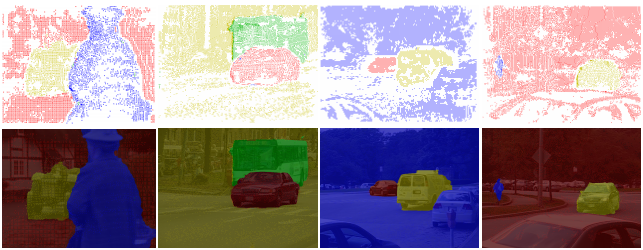
\includegraphics[height=0.28\textheight]{../images/point_traj_segm.png}
      \caption{  Sparse motion trajectories for segmentation. Results in several datasets  \cite{c34}. }
      \label{pt_segment}
   \end{figure}


The Fig. \ref{pt_segment} shows high accuracy segmentation results when using sparse motion trajectories \cite{c34}. However, to overcome 
the sparsity of the flow the authors proposed a variational method to densify the output mask. The information propagation is done 
by presenting the problem as a non-linear diffusion process that takes superpixels into account. It is expected, then, that this 
method can be precise, but slow.
In this work we propose to mix single frame graph based segmentation approaches with the idea 
of background regions tracking. However, the sparsity of point trajectories is 
overcame by using superpixels. Therefore, instead of tracking points, background regions are tracked via the novel concept of 
superpixel flow. 
We show in future sections how this extra information can be used to complement the
graph based techniques for an efficient foreground-background segmentation. 

\section{Related work}

As previously mentioned, the related work is commented mostly from an application-wise point-of-view, due to the fact that 
the object flow concept is novel. The most used approaches in the literature to mix motion estimation with scene analysis
are related to the use of this motion estimation to perform segmentation of scene \cite{c33}\cite{c34}. These works, however, depend 
intrinsically in the accuracy of the motion estimation to perform a good segmentation. Other authors have proposed to use simple 
low-order parametric motion models of the background movement, and by incorporating radial maps, obtain a frame-by-frame 
moving object segmentation \cite{c36}, in contrast with the methods that combine motion awareness with appearance information \cite{c35}. 

From other point of view, regarding the problem of large displacement motion estimation, the use of superpixels seems to provide a reliable hint. The work presented in \cite{c39} 
provides an interesting method to combine the idea of optical flow with superpixels, to obtain an optical flow method which can perform well in difficult datasets \cite{c27}. 
The full set of these ideas can lead to some conclusions towards the object flow pipeline proposal. For instance, authors have already exploited the optical flow 
to improve tracking methods. It remains unexplored to complete the cycle by improving the optical flow with the state of the tracker. Moreover, these works have shown 
that the use of superpixels can be combined with motion estimation to obtain both an object based segmentation and the enhancement of the motion itself.

On the other hand, other authors had used the optical flow constraints to track objects, 
which is, up to some extent, the inverse problem proposed for the object flow \cite{c37}. Some authors went further in this sense, to create specialized trackers 
for deformable objects by combining model based tracking with the optical flow constraint \cite{c38}. Even when \cite{c38} is very interesting for video editing 
tasks, the approach is limited by the availability of the mesh model. In this sense, the object flow proposal is more generic, and thus, more adequate for this kind 
of applications. Fig. \ref{soa1} shows some results of \cite{c38} for the video edition tasks that can also be approached with the object flow. These results are obtained in 
a controlled environment without long range motion.

   \begin{figure}[thpb]
      \centering
      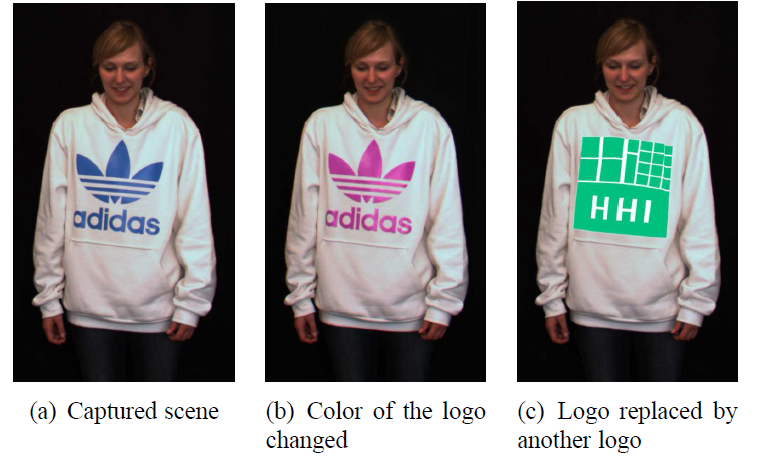
\includegraphics[width=0.75\textwidth]{../images/soa_app.png}
      \caption{  Video edition with the method in  \cite{c38}. }
      \label{soa1}
   \end{figure}

In the same line of applications, an interesting work is the Unwrap Mosaics \cite{c41} which is a very different way to approach the video edition task. 

   \begin{figure}[thpb]
      \centering
      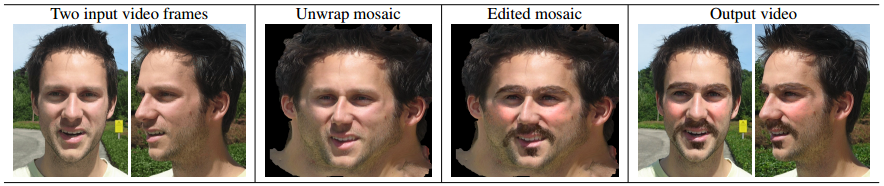
\includegraphics[width=1.00\textwidth]{../images/soa_app2.png}
      \caption{  Video edition with the method in  \cite{c41}. }
      \label{soa2}
   \end{figure}

The Unwrap Mosaics \cite{c41}, is based in a new 
video representation, which is presented by defining a 2D-2D transformation supported in a segmentation mask (given by hand), and it is used to apply the desired editing in the 
interest object, and then, given the computed mapping, the edition can be back propagated to the initial sequence. Fig. \ref{soa2} shows the video edition pipeline derived from 
this method. However, as it relies in precomputed segmentation and point trajectories, the Unwrap Mosaics can be mixed with the Object Flow pipeline to provide a robust and 
complete video edition framework. 

The object flow pipeline is, then, explained in detail in following sections. Some concepts 
are introduced first however. For instance, the superpixel flow and its mathematical 
modelling are deeply exposed in the next section. The proposed segmentation method 
is also explained later, as part of the object flow pipeline.
